\section{Explorative Analysis}
The dataset contains a mix of different breeds of cats and dogs.
The images are very diverse in terms of size, orientation, lighting, focus, and resolution.
Also, the images are taken from different angles and distances.
The images are mostly around 200-500 pixels width/height and are all in color, meaning they have 3 color channels.
In Figure \ref{fig:cats_dogs}, examples of cats and dogs from the dataset are shown.
\begin{figure}[H]
    \vspace*{-0.7cm}
    \centering
    \subfloat[][Cats]{%
        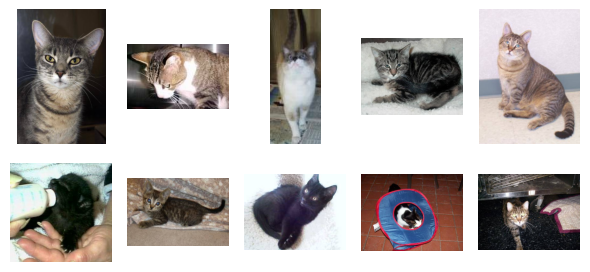
\includegraphics[width=0.48\textwidth]{figures/cats.png}\label{fig:cats}}\hspace{0.4cm}
    \subfloat[][Dogs]{%
        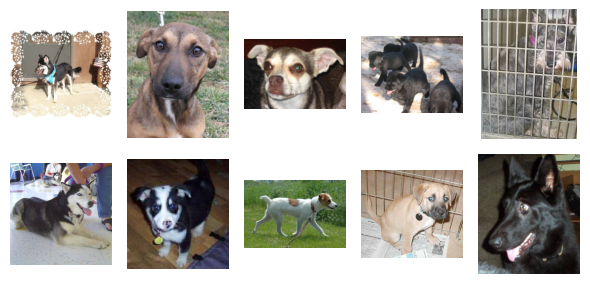
\includegraphics[width=0.48\textwidth]{figures/dogs.png}\label{fig:dogs}}
    \caption{Sample images of cats and dogs from the dataset.}
    \label{fig:cats_dogs}
    \vspace*{-0.7cm}
\end{figure}

From the images, clearly, cats and dogs have different features that can be used to distinguish between them.
For example, cats have generally shorter faces often with triangular ears and pointed noses,
while dogs generally have longer snouts and have more different ear shapes.
Moreover, the eyes of cats are generally more sharp-shaped, while dogs have rounder eyes. The goal is therefore to create a model that can learn some of these features.